% =============================================================================
% sections/s03b-framing2.tex
% 覆盖原文：p.19 "Summary so far." —— p.24 "…larger moduli space of flat connections."
% 内容：3.3 正规化与标架化、3.4 威尔逊圈与评注；编号公式 (3.25)–(3.32)，图 3，脚注 7
% 底本页面图像：work/pages/p19.png–p24.png（公式、脚注、图注均已回图核对）
% =============================================================================

% ==== 原文 p.19 ====
\subsection{正规化与标架化}\label{sec:3.3}

% 原文标题：Summary so far.
\paragraph{小结至此} 我们在 \S\ref{sec:3.1} 里搭起规范丛的几何，引入陈--西蒙斯作用量 \eqref{eq:3.3}，并借大规范变换讨论它的量子化。到 \S\ref{sec:3.2}，我们写下纯陈--西蒙斯理论的配分函数 \eqref{eq:3.8}，又尝试用鞍点法求它：在大 $k$ 下把作用量围绕一个平坦联络展开，如 \eqref{eq:3.12}。

% ==== 原文 p.20 ====
随后我们选定度规、固定规范、引入鬼场，借助那些二次型构成规范固定作用量的算子，算出所得的高斯型路径积分。结果是 \eqref{eq:3.17}：一个行列式之比，其绝对值 $T_\alpha$ 是拓扑不变量。相位要微妙得多，最终用 $\eta$ 不变量 \eqref{eq:3.22} 写了出来。可惜 $\eta[A^{(\alpha)}]$ 不是拓扑不变量，因为它依赖 $L_-$，从而依赖 $M$ 的度规。指标定理给出 \eqref{eq:3.24}，把局面改善了一步：$\mathcal{Z}$ 里只剩 $\eta[0]$ 不是拓扑不变量。

% [Tutor Note: 含糊点] 行列式之比的绝对值是拓扑不变量，依据是 Schwarz [14] 的雷–辛格挠率；定义要求无零模。
\begin{yizhu}[含糊点]
作者只说行列式之比的绝对值 $T_\alpha$ 是拓扑不变量，未给依据。这正是雷–辛格挠率（Ray--Singer torsion）的陈述：对平坦联络，算子 $\Delta$ 与 $L_-$ 的行列式之比（按射线意义）只依赖和乐，与度规无关；而定义这个比值要求算子无零模，即本片段末段「行列式必须非零」那条告诫。术语与构造见 Schwarz \cite{schwarz1978}。
\end{yizhu}

转向 $\eta[0]$：平凡联络 $A^{(\alpha)}=0$ 把协变导数退化成普通导数，$D_\mu=\partial_\mu$。于是 $L_-$ 成为 $d=\dim G$ 个相同副本的直和，每个副本都是「引力」算子 $D_-=(\star\dd+\dd\star)_{\text{odd}}$；叫它「引力」，只因它只依赖 $M$ 的度规。因此可写 $\eta[0]=d\eta_g$，其中 $\eta_g=\eta_g$ 是 $D_-$ 在 $A^{(\alpha)}=0$ 处的 $\eta$ 不变量。接着我们希望把 \eqref{eq:3.24} 里的整体相位 $\Lambda\equiv\exp\bigl(\tfrac{id\pi}{2}\eta_g\bigr)$ 也表成拓扑不变量，可这里运气用光了。

% [Tutor Note: 原文疑误] p.20 图像作 η_g=η_g，同一符号自等，疑漏写「平凡联络处」的标记；照录不改。
\begin{yizhu}[原文疑误]
p.20 图像原文作 $\eta_g=\eta_g$：同一符号自等，等于什么也没说。对照 \eqref{eq:3.23} 用 $\eta[0]$ 记平凡联络处的 $\eta$ 值，此处疑漏了标记，应读作 $\eta_g=\eta_g[0]$（或 $\eta_g\equiv\eta_g^{(0)}$），即 $D_-$ 在 $A^{(\alpha)}=0$ 处的 $\eta$ 值。正文照录不改；读者把第二个 $\eta_g$ 读成「平凡联络处的 $\eta_g$」即可。
\end{yizhu}

% 原文标题：Philosophy of failure.
\paragraph{失败的哲学} 要紧的是认清一点：我们起步时拿的是拓扑量，可无论怎么正规化、怎么算，都躲不开引入度规。广义协变性本是陈--西蒙斯作用量的「经典」对称性；量子理论的任何正规化都会破坏它，于是理论该有反常——果然，我们马上会看到一个，叫「标架反常」。不过更紧迫的是：最终答案依赖度规。这不奇怪：\eqref{eq:3.13} 里为定规范而加的那些项显式耦合度规，所以我们的计算只能对到作用量中这类「引力」项的效果为止。真正令人意外的，也许是：我们几乎把这些效果全消掉了，只剩整体相位因子 $\Lambda=\exp\bigl(\tfrac{id\pi}{2}\eta_g\bigr)$ 一项。

要补救，就得往作用量里加一个补偿项，精确抵消我们引入的引力效果。这个做法与重整化的想法一致：任意两种正规化之差，必是作用量中某个局域抵消项。这里我们需要一个只由 $M$ 上度规 $g$ 构造的抵消项 $\mathcal{C}[g]$，使得把 $i\mathcal{C}[g]$ 加进作用量后，对 $\mathcal{Z}$ 的唯一影响就是把 $\mathcal{C}[g]$ 加到相位 $\frac{d\pi}{2}\eta_g$ 上。我们约定：只要和 $\frac{d\pi}{2}\eta_g+\mathcal{C}[g]$ 是拓扑不变量，就说 $\mathcal{C}[g]$「精确抵消」了 $\eta_g$ 的引力效果——因为那时它不再依赖度规。

% 原文标题：The gravitational counterterm.
\paragraph{引力抵消项} 该往作用量里加什么，也许不好想。一个自然的猜测是引力陈--西蒙斯作用量：仿照 $\SCS$ 写，只把主 $G$-联络 $A$ 换成 $M$ 上的自旋联络 $\omega$：

\begin{equation}\tag{3.25}\label{eq:3.25}
  I[g] \equiv \frac{1}{4\pi}\int_M \Tr\left(\omega\wedge\dd\omega + \frac{2}{3}\,\omega\wedge\omega\wedge\omega\right).
\end{equation}

% [Tutor Note: 易错点] (3.25) 的 1/4π 是单位能级归一化；ω 是旋量丛 Levi-Civita 联络，取值 so(3)≅su(2)；2/3 由 dTr(...)=Tr(R∧R) 定住。
\begin{yizhu}[易错点]
\eqref{eq:3.25} 的 $1/4\pi$ 与 \eqref{eq:3.3} 的 $k/4\pi$ 同源，相当于取单位能级 $k=1$，不能把 $k$ 再乘进去。$\omega$ 也不是任意的 $\mathrm{SU}(2)$ 规范场：它是旋量丛上的列维–奇维塔联络，取值在 $\mathrm{so}(3)\cong\mathrm{su}(2)$，位形由度规 $g$ 唯一固定，故 $I[g]$ 只是 $g$ 的泛函。三次项系数 $2/3$ 由 $\dd\,\Tr(\omega\wedge\dd\omega+\frac{2}{3}\omega\wedge\omega\wedge\omega)=\Tr(R\wedge R)$ 定住；这一归一化使 $I[g]$ 的变分成为陈--韦伊密度，标架变换下它才只差 $2\pi$ 的整数倍。
\end{yizhu}

粗略地说，可以把 $\omega$ 想成 $M$ 上的列维–奇维塔联络。更准确、也更有启发的看法是：$\omega$ 是 $M$ 的旋量丛上的列维–奇维塔联络。

% ==== 原文 p.21 ====
多亏 3 维的一个幸运事实——$\mathrm{Spin}(3)$ 是 $\mathrm{SO}(3)$ 的万有覆叠，且同构于 $\mathrm{SU}(2)$——这个构造立刻具体起来：$\omega$ 就是一个 $\mathrm{SU}(2)$ 规范场，而它具体的场位形（从而 $I[g]$ 的取值）只由一条「引力」要求固定：它是列维–奇维塔联络。

$I[g]$ 这一项正是我们要的关键配料。由阿蒂亚–辛格指标定理（又是它！），引力项的组合 $\Xi\equiv\frac{1}{2}\eta_g+\frac{1}{12}\frac{I[g]}{2\pi}$ 是拓扑不变量。按照上面陈述的哲学，我们应把配分函数整体相位 $\Lambda$ 里的 $\frac{\eta_g}{2}$ 换成 $\Xi$。换言之，应往作用量里加抵消项 $\mathcal{C}[g]=\frac{\pi d}{12}\frac{I[g]}{2\pi}=\frac{dI[g]}{24}$，于是 \eqref{eq:3.24} 里那个麻烦的相位成为

\begin{equation}\tag{3.26}\label{eq:3.26}
  \Lambda = \exp\left(\frac{i\pi}{2}\eta[0]\right)
        = \exp\left(\frac{id\pi}{2}\eta_g\right)
        \leadsto \exp\left(i\pi d\left[\frac{\eta_g}{2}+\frac{1}{12}\frac{I[g]}{2\pi}\right]\right)
        = \exp(i\pi d\,\Xi).
\end{equation}

% [Tutor Note: 易错点] (3.26) 中间是波浪箭头 \leadsto 而非除号；η[0]=dη_g 使相位取 +，若读成除法与 (3.27) 符号矛盾。
\begin{yizhu}[易错点]
p.21 图像上，第二个等号与右侧表达式之间是波浪箭头 $\leadsto$，不是除号（提取文本把它误认成「/」）。故 \eqref{eq:3.26} 里没有相除：由 $\eta[0]=d\eta_g$ 得 $\frac{\pi}{2}\eta[0]=\frac{d\pi}{2}\eta_g$，再把 $\frac{\eta_g}{2}$ 换成 $\Xi=\frac{\eta_g}{2}+\frac{1}{12}\frac{I[g]}{2\pi}$，相位即由 $e^{id\pi\eta_g/2}$ 变为 $e^{i\pi d\Xi}$，全程取 $+$ 号。若照字面作除法，得到 $e^{-i\pi dI[g]/(24\pi)}$，与 \eqref{eq:3.27} 括号内的 $+\frac{I[g]}{24\pi}$ 符号相反，矛盾立刻显形。
\end{yizhu}

% [Tutor Note: 含糊点] Ξ 的拓扑不变性来自 APS 指标定理 [15–17]：η 的度规依赖被 I[g] 项抵消。
\begin{yizhu}[含糊点]
$\Xi\equiv\frac{1}{2}\eta_g+\frac{1}{12}\frac{I[g]}{2\pi}$ 的拓扑不变性靠阿蒂亚–帕托迪–辛格（APS）指标定理 \cite{aps1975,aps1976a,aps1976b}。带边 4-流形上的指标定理把椭圆算子的指标写成内部密度减去边界项 $\frac{\eta+h}{2}$；在自旋（或符号差）算子情形，$\eta_g$ 的度规依赖恰与 $\frac{1}{12}\frac{I[g]}{2\pi}$ 的变化相消（$I[g]$ 的变分给出 $\Tr(R\wedge R)$ 型密度），组合便只余拓扑信息。作者写 (again!) 是提醒：\eqref{eq:3.23} 已用过同一定理。
\end{yizhu}

千呼万唤，单圈配分函数终于完全拓扑化：

\begin{equation}\tag{3.27}\label{eq:3.27}
  \mathcal{Z} = \exp\left(i\pi d\left[\frac{\eta_g}{2}+\frac{I[g]}{24\pi}\right]\right)
  \sum_{\alpha}\exp\left[i\left(k+\frac{c_2(G)}{2}\right)I[A^{(\alpha)}]\right]T_\alpha .
\end{equation}

% 原文标题：Framing.
\paragraph{标架化} 上面的讨论略去了一个关键却技术性的点：$I[g]$ 有一种几何上的含糊，很像 $\SCS$ 失去规范不变性的那种失效。众所周知 \cite{parker1984}：每个有向 3-流形都容许其切丛的一个平凡化；这样的平凡化叫标架（framing）。同样众所周知 \cite{milnor1974}：每个有向 3-流形都容许自旋结构。（这保证 \eqref{eq:3.25} 之后对 $\omega$ 的刻画说得通。）事实上，每个标架的选择唯一决定一个自旋结构；这个选择左右旋量丛的几何，从而影响它的列维–奇维塔联络。一般的 3-流形没有标准标架，所以除非选定标架，$I[g]$ 的值没有定义。换句话说：相对于一种自旋结构，$M$ 上其他旋量丛的列维–奇维塔联络看起来像带挠率的，但没有标准办法判定其中哪个「真正」无挠。

% [Tutor Note: 含糊点] 「有向 3-流形可平行化」是可平行化定理（Steenrod [9]）；自旋结构存在见 Milnor [19]；标架→自旋结构靠 SO(3) 提升到 Spin(3)。
\begin{yizhu}[含糊点]
「每个有向 3-流形都容许切丛平凡化」是 3 维特有的结论：有向 3-流形可平行化，$w_1=w_2=0$，见 \cite{parker1984}，教材叙述见 Steenrod \cite{steenrod1951}；故自旋结构存在，见 Milnor \cite{milnor1974}。选定平凡化（标架）后，结构群从 $\mathrm{SO}(3)$ 提升到 $\mathrm{Spin}(3)\cong\mathrm{SU}(2)$，于是确定一个自旋结构——这就是正文「每个标架唯一决定一个自旋结构」的依据。换标架即换旋量丛的联络，$I[g]$ 才有歧义。
\end{yizhu}

$I[g]$ 没有明确取值，我们最多只能描述标架变换下 $I[g]$（从而 $\mathcal{Z}$）怎么变。实际上，任两个标架给出的 $I[g]$ 相差 $2\pi$ 乘一个整数 $s$，$s$ 度量两者之间相对「扭转」的次数。（变换律 $I[g]\longrightarrow I[g]+2\pi s$ 与陈--西蒙斯作用量在大规范变换下的行为 $\SCS\longrightarrow\SCS+2\pi kw$ 直接类似。）把标架平移 $s$ 个单位，\eqref{eq:3.27} 表明配分函数变为

\begin{equation}\tag{3.28}\label{eq:3.28}
  I[g]\longrightarrow I[g]+2\pi s
  \quad\Longrightarrow\quad
  \mathcal{Z}\longrightarrow\exp\left(\frac{2\pi isd}{24}\right)\mathcal{Z}.
\end{equation}

% [Tutor Note: 易错点] (3.27)–(3.28) 的 d=dim G 来自 η[0]=dη_g；分母 24 由 12·2π 合成；d=24 时 e^{2πis}=1。
\begin{yizhu}[易错点]
$d$ 是 \eqref{eq:3.27} 里 $\eta[0]=d\eta_g$ 带出的规范群维数，$d=\dim G$（伴随表示维数），不是能级 $k$，也不是对偶考克斯特数；分母 $24$ 由 $12\cdot2\pi$ 合成。$I[g]\longrightarrow I[g]+2\pi s$ 使 $e^{i\pi dI[g]/(24\pi)}$ 多出 $e^{2\pi isd/24}$。\eqref{eq:3.32} 之后的 $\mathrm{SU}(5)$ 例中 $d=24$，故 $e^{2\pi is}=1$，标架依赖整体消失；若把 $24$ 误当 $24\pi$、或把 $d$ 误当 $c_2(G)=4$，就会错判仍有标架反常。
\end{yizhu}

% ==== 原文 p.22 ====
\subsection{威尔逊圈与评注}\label{sec:3.4}

% 原文标题：An abelian example.
\paragraph{一个阿贝尔例子} 在非阿贝尔陈--西蒙斯理论里纳入威尔逊圈，即按 \eqref{eq:3.7} 计算 $\mathcal{Z}(M,L)$，很难，先放一放。这里重回 \S\ref{sec:2.2} 讨论过的阿贝尔情形：$M=S^3$，$G=\mathrm{U}(1)$，作用量取 \eqref{eq:2.1}。取 $r$ 条互不相交、有向、闭的曲线 $\gamma_1,\dots,\gamma_r$，其并为链环 $L$；再取整数 $n_1,\dots,n_r$，扮演 $\mathrm{U}(1)$ 不可约表示的角色。考虑威尔逊链环

\begin{equation}\tag{3.29}\label{eq:3.29}
  W[L] \equiv \prod_{a=1}^{r}W_a[\gamma_a]
  = \prod_{a=1}^{r}\exp\left(n_a\oint_{\gamma_a}\dd x_a^\mu A_\mu\right).
\end{equation}

（\eqref{eq:3.6} 里的路径排序符号在这里不需要，因为理论是阿贝尔的。）推广 \S\ref{sec:2.2} 的结果，$W[L]$ 的期望值可写成

\begin{equation}\tag{3.30}\label{eq:3.30}
\begin{aligned}
  \langle W[L]\rangle
  &\equiv \frac{1}{\mathcal{Z}}\int\mathcal{D}A\,W[L]\,e^{i\SCS[A]}
  = \exp\left(\frac{i}{2k}\sum_{a,b=1}^{r}n_a n_b
    \oint_{\gamma_a}\dd x_a^\mu\oint_{\gamma_b}\dd x_b^\nu\,
    \varepsilon_{\mu\nu\rho}\frac{(x_a-x_b)^\rho}{|x_a-x_b|^3}\right)\\
  &= \exp\left(\frac{2\pi i}{k}\sum_{a,b=1}^{r}n_a n_b\,\Phi[\gamma_a,\gamma_b]\right),
\end{aligned}
\end{equation}

其中 $x_a^\mu$ 与 $x_b^\nu$ 是 $S^3$ 上包含 $L$ 的某区域的局部坐标，$\Phi[\gamma_a,\gamma_b]$ 是 $\gamma_a$ 与 $\gamma_b$ 通常的高斯环绕数，由 \eqref{eq:2.19} 定义。

% [Tutor Note: 易错点] (3.30) 两行系数 i/2k 与 2πi/k 相差 4π，即高斯环绕积分的 1/4π；(3.31) 指数是 n_a^2 不是 2n_a^2。
\begin{yizhu}[易错点]
\eqref{eq:3.30} 两行系数 $\frac{i}{2k}$ 与 $\frac{2\pi i}{k}$ 相差 $4\pi$，正是高斯环绕积分的归一化 $\Phi=\frac{1}{4\pi}\oint\oint\varepsilon_{\mu\nu\rho}\frac{(x_a-x_b)^\rho}{|x_a-x_b|^3}\dd x_a^\mu\dd x_b^\nu$（见 \eqref{eq:2.19}），$\Phi$ 因此是无量纲的环绕数，两条互不相交的闭曲线之间取整数值。\eqref{eq:3.31} 的指数是 $n_a^2$ 而非 $2n_a^2$：有序对 $(a,a)$ 在双重和里只出现一次，$\Phi_s[\gamma_a]$ 平移 $t$ 只贡献一项 $n_a^2t$。
\end{yizhu}

% 原文标题：The self-linking number.
\paragraph{自环绕数} 当 $a=b$ 时，自环绕数 $\Phi_s[\gamma_a]\equiv\Phi[\gamma_a,\gamma_a]$ 发散。\S\ref{sec:2.2} 里我们用最省事的办法绕开：干脆丢掉这类自相互作用项。但正规化这些无穷大还有更漂亮的一招：沿每条纽结 $\gamma\subset L$，选一个处处与 $\gamma$ 正交的向量场。这样的选择叫 $\gamma$ 的标架（framing），与我们在 \S\ref{sec:3.3} 里发展的 3-流形标架一脉相承。\footnote{这种标架概念等价于为纽结的切丛 $T\gamma$ 选定一个平凡化，因此按我们最初的字面意思，它也定义了 $\gamma$ 作为 1-流形的标架。} 接着把 $\gamma$ 沿这个向量场稍稍平移，加粗成一条带子，如图 \ref{fig:framing} 所示。带子以 $\gamma$ 与一条新纽结 $\gamma'$ 为边界；我们定义自环绕数 $\Phi_s[\gamma]$ 为 $\Phi[\gamma,\gamma']$。

% 原文标题：Change of framing.
\paragraph{标架变换} 这个规定显然依赖延拓 $\gamma$ 所用向量场的拓扑类，而且一般使 $\Phi_s[\gamma]\neq0$。在 $S^3$ 里，每条纽结其实都有标准标架：要求自环绕数为零即可，\S\ref{sec:2.2} 选的正是它。但一般情形并非如此：任意 3-流形中的纽结没有标准标架可选。正如对 $\mathcal{Z}$ 那样，我们在这里也只满足于一条规律，管住 $\Phi_s[\gamma]$ 与 $\langle W[L]\rangle$ 在标架变换下怎么变。所幸指标定理保证：两种不同标架给出的自环绕数相差整数次扭转 $t$，如图 \ref{fig:framing} 所示。

% ==== 原文 p.23 ====
当纽结 $\gamma_a$ 的标架平移 $t$ 个单位时，\eqref{eq:3.30} 告诉我们 $\langle W[L]\rangle$ 变为

\begin{equation}\tag{3.31}\label{eq:3.31}
  \Phi_s[\gamma_a]\longrightarrow\Phi_s[\gamma_a]+t
  \quad\Longrightarrow\quad
  \langle W[L]\rangle\longrightarrow
  \exp\left(\frac{2\pi itn_a^2}{k}\right)\langle W[L]\rangle.
\end{equation}

数学上，\eqref{eq:3.28} 与 \eqref{eq:3.31} 说明 $\mathcal{Z}$ 与 $\langle W[L]\rangle$ 是标架化流形的拓扑不变量。物理上，它们描述一种标架反常，来源是引力耦合。

\begin{figure}[htbp]
  \centering
  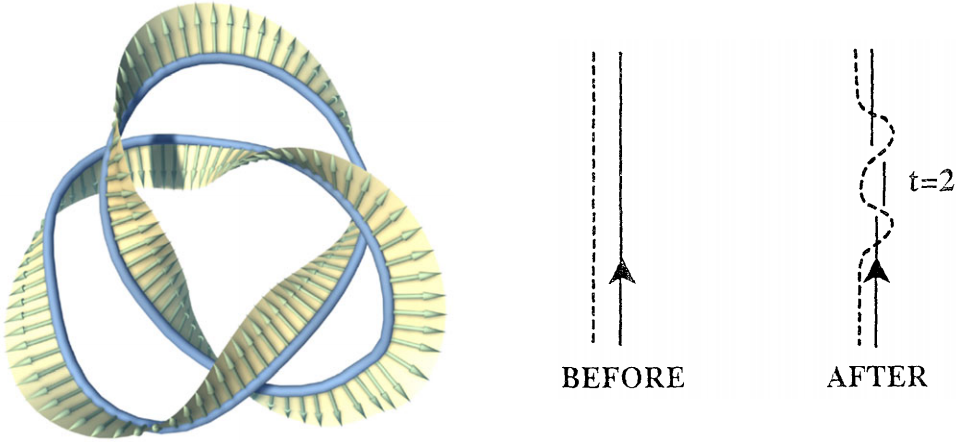
\includegraphics[width=0.85\textwidth]{figures/fig3_trefoil_framing.png}
  \caption{左：三叶结标架的一个选择，就是一个与它正交、把它「框住」的向量场 \cite{elhamdadi2020}。右：标架变换可以看成 $\gamma'$ 相对 $\gamma$ 的一次扭转 \cite{witten1989}。（原文 Figure 3，原文 p.23）}
  \label{fig:framing}
\end{figure}

% 原文标题：Examples and caveats.
\paragraph{例子与告诫} 收尾时，把展开理论过程中漏掉的评论、例子与警告一并补上。先看几个显式配分函数。对 $M=S^2\times S^1$，任意规范群 $G$ 都有 $\mathcal{Z}=1$。对 $M=S^3$，规范群 $G=\mathrm{U}(1)$ 时可用结果 \eqref{eq:3.30}：取空链环，相位为零，故 $\mathcal{Z}=1$。对 $M=S^3$ 与非阿贝尔 $G$，唯一的平坦联络是平凡联络 $A^{(\alpha)}=0$。有人或许想套用 \eqref{eq:3.27}，但（下面会讨论）它在这里其实失效。$G=\mathrm{SU}(2)$ 的实际结果及其大 $k$ 标度行为是

\begin{equation}\tag{3.32}\label{eq:3.32}
  \mathcal{Z} = \sqrt{\frac{2}{k+2}}\,\sin\left(\frac{\pi}{k+2}\right) \sim k^{-3/2}.
\end{equation}

注意 $c_2(\mathrm{SU}(2))=4$，所以这里出现的因子 $k+2$ 其实就是单圈下「重整化」过的陈--西蒙斯能级 $k+\frac{c_2(G)}{2}$。另外，有件颇有意思的小事：规范群 $G=\mathrm{SU}(5)$ 有 $d=\dim G=24$，把它代入 \eqref{eq:3.28}，$\mathcal{Z}$ 对 $M$ 的标架的依赖就彻底消失了。

最后，我们指出 \S\ref{sec:3.2} 里一条重要的告诫：算子 $\Delta$ 与 $L_-$ 的行列式必须非零，\eqref{eq:3.17} 的一切推论才说得通。事实上，这些算子非奇异，当且仅当 $A^{(\alpha)}$ 平凡化所有德拉姆上同调群 $H^n_{\mathrm{dR}}(M,E)$。这些对象来自一个观察：在平坦丛上，$[D_\mu,D_\nu]=F_{\mu\nu}=0$ 蕴含 $D\circ D=0$。于是协变导数是由平坦联络 $A^{(\alpha)}$ 扭出的上边缘算子，上同调定义为 $H^n_{\mathrm{dR}}(M,E)=\bigl(\ker D|_{\Omega^n(M,E)}\bigr)\big/\bigl(\operatorname{im}D|_{\Omega^{n-1}(M,E)}\bigr)$。让我们的结果失效，最省事的办法

% ==== 原文 p.24 ====
是找一个 $H^0(M,E)\neq0$ 的情形。一旦如此，算子 $\Delta$ 与 $L_-$ 就有零本征值，辅助场 $\phi$、$\bar c$、$c$ 就有零模，定规范随之变复杂。$M=S^3$ 时正是如此，那里唯一的平坦联络是平凡联络。具体说，$H^0(M,E)=\ker\dd|_{C^\infty(M,E)}=E\neq0$，即常值映射 $M\to E$ 的集合。所以，虽有「平凡」之名，平凡联络却惹来大麻烦。最后我们注意到：若 $H^1_{\mathrm{dR}}(M,E)\neq0$，平坦联络便不孤立、数目也不再有限，而是落在一个更大的平坦联络模空间里。

% =============================================================================
% 交付汇报（片段 s03b）
% * 覆盖原文 p.19–p.24（至 "…larger moduli space of flat connections." 止），
%   编号公式 (3.25)–(3.32) 共 8 个（\tag 锁定、顺序照原文），图 3，脚注 7。
% * 译注 8 条：易错点 4 条（(3.25) 的 1/4π 与 ω 取值；(3.26) 相位代数与波浪箭头；
%   (3.27)–(3.28) 的 d=dim G 与 24；(3.30)–(3.31) 的 4π 归一化与 n_a^2），
%   含糊点 3 条（APS [15–17]、[18][19]+[9]、Schwarz [14] 的 Ray–Singer 挠率），
%   原文疑误 1 条（p.20 的 η_g=η_g）。
% * SPEC §10 裁定：
%   第 10 条成立：p.20 图像确作 "η_g = η_g"，照录 + 批注。
%   第 11 条不成立：p.21 图像 (3.26) 中第二个等号后是波浪箭头（\leadsto），
%     提取文本误作「/」；相位符号与 (3.27) 一致，无矛盾，故按图像录为箭头、
%     不写「原文疑误」批注。
%   第 12 条已核，无误：d=dim G=24 时 e^{2πis}=1，标架依赖消失。
% * 另见存疑：p.23 "all of the the de Rham cohomology groups" 重复一个 the
%   （中文不可见，未加注，报 Lead）；(3.30) 第二行与第一行系数之差 4π 已在译注说明。
% =============================================================================
